\documentclass[12pt]{amsart}
\usepackage[margin = 1in]{geometry}
\usepackage[shortlabels]{enumitem}
\usepackage{graphicx}
\usepackage{subfig}
\usepackage{hyperref}
\usepackage{commath}

\newtheorem{theorem}{Theorem}
\newtheorem{lemma}{Lemma}
\theoremstyle{definition}
\newtheorem{definition}{Definition}
\newtheorem{asmp}{Assumption}


\begin{document}
\title[New Valuation Measure Equity-Linked Annuities]{A New Stock Market Valuation Measure with Applications to Equity-Linked Annuities}

\author{Andrey Sarantsev}
\address{University of Nevada in Reno, Department of Mathematics and Statistics}
\email{asarantsev@unr.edu}

\begin{abstract} We propose a new stock market valuation measure. We use the USA stock market data from 1871. We split total returns into three components: earnings growth, dividend yield, and valuation change. The first two components are fundamental, the third is speculative. We treat earnings growth as exogenous. Combining the other two components gives us a new valuation measure, which fits autoregression of order 1 with Gaussian innovations, centered at 4.6\%. Therefore, long-term total returns equals long-term earnings growth plus 4.6\%. We confirm the classic 4\% withdrawal rule for investing in stocks: A retiree should invest in stocks and withdraw 4\% of initial wealth after adjusting for inflation. This is useful for equity-linked annuities, which invest retiree's savings used for annuity purchase into the stock market. 
\end{abstract}

\keywords{Autoregression, block bootstrap, strong mixing, Central Limit Theorem, total returns, earnings growth, dividend yield. Classification (JEL): C22, C58, G17; (AMS 2020): 60F05, 60G10, 62J05, 62M10, 62P05, 62P20, 91B84}

\maketitle

\thispagestyle{empty}

\section{Introduction} 

\subsection{Price-earnings ratio} Forecasting future stock market returns is a major area of study in financial mathematics. There is a long tradition of using different versions of the price-earnings ratio, abbreviated as the {\it P/E ratio}. A stock market or portfolio with high P/E ratio is deemed overpriced, with bearish growth prospects. Conversely, a stock market of portfolio with low P/E ratio is considered attractively underpriced. Robert Shiller designed a {\it cyclically adjusted price-earnings} (CAPE) ratio which takes 10-year averaged inflation-adjusted earnings in the denominator. He collected US stock market data starting from 1871, which we use in this article. 

An advantage of averaged earnings is smoothing out business cycle fluctuations. During recessions, earnings temporarily plummet, but the impact upon long-term earnings prospects is small. Thus P/E ratio can increase during recessions, but this does not mean that the stock market is overpriced. The CAPE ratio solves this problem. 

This CAPE ratio has significant predictive power for future inflation-adjusted stock market returns (including dividends and price changes). We use the 5-year version here, which is not significantly different from the classic 10-year version. The CAPE graph (together with its total returns-adjusted version, see below) is on~\textsc{Figure}~\ref{fig:cape}. 

\subsection{The new bubble measure} There is evidence that in the past few decades, companies prefer to distribute earnings to shareholders via buybacks, rather than dividends. This pushes price upward and increases these P/E ratios, but does not necessarily affect total returns (which combine both price changes and dividend payouts). We consider another valuation measure, which we call {\it the bubble measure}. We compute it as follows.

Long-term stock returns are equal to long-run earnings growth plus long-run dividend yield. Now, from annual total returns, subtract the annual earnings growth. We compute the latter using 5-year inflation-adjusted trailing earnings. This is called {\it implied dividend yield} $\Delta(t)$. Annual total returns are on average 6--7\%, but real earnings growth is 2\% annually. Thus the long-term average $c$ of implied dividend yield is 4--5\%. 

This is consistent with the observation that pure return on capital in traditional agrarian societies (without economic and therefore earnings growth) is 4--5\%. However, implied and actual dividend yield are not always equal. In the 19th century, this is the actual dividend yield. In the 21st century, the actual dividend yield is 2--3\%. Thus we think that $\Delta(t)$ is a more accurate valuation measure than the actual dividend yield. 

If $\Delta(t) > c$ then the market became more overpriced in year $t$. Conversely, if $\Delta(t) < c$, then the market became more underpriced in year $t$. Thus the difference $\Delta(t) - c$ is considered the annual change in this bubble measure. We sum all these past differences for $t = 1, \ldots, s$ to get the current {\it bubble measure} $H(s)$. This bubble measure is our version of CAPE: When it is high, then the market is overpriced.  This bubble measure $H(t)$ satisfies AR(1) (autoregression of order 1) with Gaussian innovations (residuals) $\varepsilon(t)$:
\begin{equation}
\label{eq:ar-initial}
H(t) - h = b(H(t-1) - h) + \varepsilon(t)
\end{equation}
These two valuation measures (CAPE and the bubble measure) are close until the last 20 years, then they diverge. You can see two measures on \textsc{Figure}~\ref{fig:compare}. As of January 2022, the CAPE shows that the market is overpriced, but the bubble measure shows that it is underpriced. As we discussed earlier, this is due to recently changed dividend payout policy.

\subsection{Equity-linked annuities and withdrawal rates} We apply our results for retirement planning. A retiree needs to withdraw certain amounts each year from wealth. A major problem in finance is {\it retirement planning}: How much a retiree can withdraw per year to keep income more or less stable, and still preserve wealth? Wealth funds and university endowments face a related problem; the difference is that, unlike the retiree, they wish to preserve the wealth forever, and not for 20--30 years. 

A classic withdrawal rule is 4\%. It exists in two versions: (a) {\it constant:} Withdraw inflation-adjusted 4\% of initial wealth; (b) {\it proportional:} Withdraw 4\% of current wealth. The first rule ensures constant stream of payments, but could deplete wealth up to zero ({\it ruin}, or {\it bankruptcy}). A financial planner must ensure that the ruin probability is small. The second rule ensures that there is no ruin, but income could fluctuate with the market. 

We can view this withdrawal rule as an {\it equity-linked annuity}. Annuities are streams of regular future payments, bought at some time by a client from an insurance company. Often, annuities invest conservatively: in Treasury bonds or highly rated corporate and municipal bonds. Thus the annual rate for annuity (fraction of original price paid annually) is approximately equal to long-term Treasury or investment-grade corporate rates. As of this writing, these are below or barely above the projected future inflation. Many retirees and investors would not be satisfied with this performance. 

An alternative would be investing money obtained from selling an annuity in the stock market. This is an {\it equity-lined annuity}. For example, the capital can be invested in a Standard \& Poor 500 mutual index fund. This would be called {\it equity-indexed annuity}. Stocks are much more risky than aforementioned bonds, but have the potential for much higher future returns. Below we show that 4\% or even 5\% annual rate is achievable with only small risk of default (i.e. not fulfilling these obligations). Life expectancy does not matter: in fact, below we can assume the time horizon is infinite. We refer to textbooks \cite[Chapter 8]{ActuarialBook} and \cite{FengBook}, as well as to articles \cite{Anna, Guarantees, IndexedAnnuity}.

\subsection{Organization of the article} In Section 2, we explain the financial background: stock market index, earnings, dividends. We provide literature review, and quote popular economics and financial books to motivate this research. 

Section 3 is devoted to statistical analysis of annual stock market data 1871--2022. We fit the authoregressive model AR(1) model for the bubble measure. Using one linear regression, we determine 3 parameters: Long-term implied dividend yield $c$, and the AR(1) parameters in~\eqref{eq:ar-initial}: Long-term average $h$ of the bubble measure, and the autoregression coefficient $b$. We analyze residuals $\varepsilon(t)$ in~\eqref{eq:ar-initial}. We fail to reject the hypothesis that they are Gaussian independent identically distributed. Thus we assume $\varepsilon(t) \sim \mathcal N(0, \sigma^2)$ i.i.d. We reject the unit root hypothesis. That is, show that the AR(1) from~\eqref{eq:ar-initial} is mean-reverting; $b \in (0, 1)$. 

Section 4 is devoted to theory. We start from two processes: AR(1) and the fundamental process (which in real data corresponds to 5-year averaged earnings). From these, we reconstruct total real returns and real earnings growth. We study theoretical properties: Strong Law of Large Numbers in Theorem~\ref{thm:SLLN} and the Central Limit Theorem in Theorem~\ref{thm:CLT}. 

In Section 5, we study retirement planning. We consider an equity-indexed annuity investing in S\&P 500 index fund and making annual withdrawals. We state several results (Theorem~\ref{thm:withdrawal} and some computations) for withdrawal strategies, both proportional (fractions of current wealth) and constant (fractions of initial wealth, inflation-adjusted). In particular, we verify the classic 4\% withdrawal rule (withdrawing annually 4\% of the inflation-adjusted initial wealth). But the 5\% rule is no longer safe. 

Section 6 is devoted to conclusions and suggestions for future research.

The Appendix contains proofs of our results. The \texttt{GitHub} repository \texttt{asarantsev/IDY} contains our Python code and data.

\subsection{Acknowledgements} The author is thankful to his University of Nevada, Reno students Akram Reshad, Taran Grove, Erick Luerken, Tran Nhat, and Michael Reyes for useful discussion. The author thanks the Department of Mathematics \& Statistics at the University of Nevada, Reno, for welcoming atmosphere for research.

%\subsection{Funding Sources} The author did not receive any funding. 

%\subsection{Conflict of Interest} The author declares no conflict of interest. 

\section{Background}

\begin{figure}[t]
\subfloat[Index]{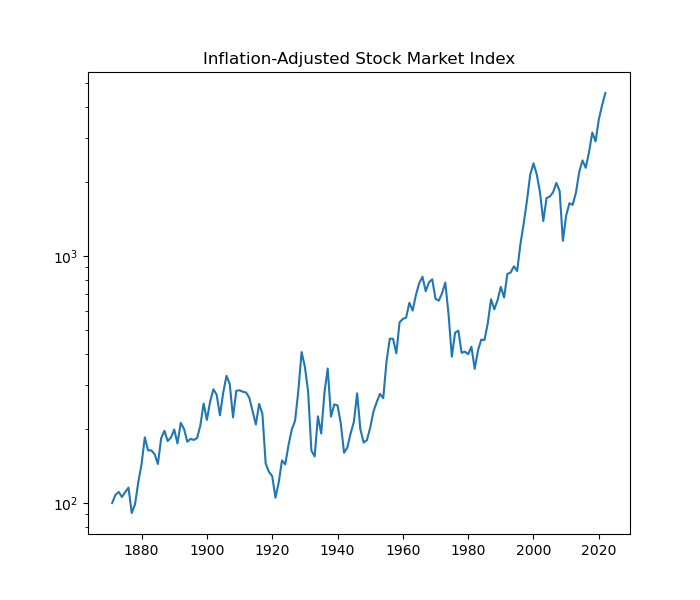
\includegraphics[width = 8cm]{index.png}}
\subfloat[Wealth, 1871 = 1\$]{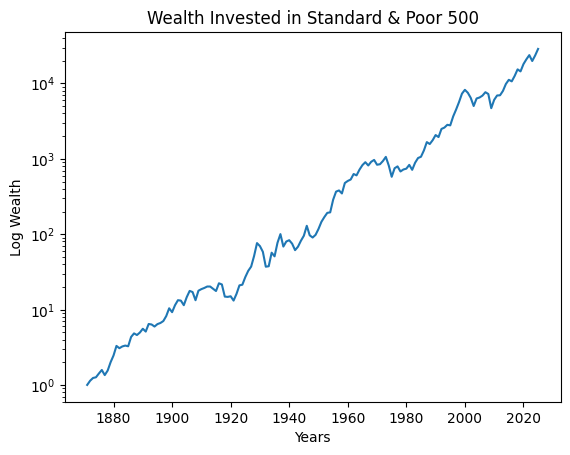
\includegraphics[width = 8cm]{wealth.png}}
\caption{Inflation-adjusted index and wealth 1871--2022}
\label{fig:index}
\end{figure}

\subsection{Sources of stock market returns} The long-run total returns of a stock portfolio, or an individual stock, or the entire stock market, are composed of three parts: dividend yield (dividends paid last year divided by the current price of a stock), earnings growth, and changes in the {\it P/E ratio}, or {\it price-to-earnings ratio}. For the market as a whole (measured by the Standard \& Poor 500 or any other index), the P/E ratio and is computed as the sum of P/E ratios of individual stocks, weighted by market capitalizations (total market value) of stocks.  or, equivalently, the ratio of the total market value of all these stocks to their total earnings over the last year. To quote the book \cite[pp.324--325]{RW12}:

\begin{quote}
Very long-run returns from common stocks are driven by two critical factors: the dividend yield at the time of purchase, and the future growth rate of earnings and dividends. In principle, for the buyer who holds his or her stock forever, a share of common stock is worth the present, or discounted value of its stream of future dividends. Recall that this discounting reflects the fact that a dollar received tomorrow is worth more than a dollar received today. [...] The discounted value of this stream of dividends (or funds returned to shareholders through stock buybacks) can be shown to produce a very simple formula for the long-run total return for either an individual stock or the market as a whole: Long-run equity return = initial dividend yield + growth rate. [...] Over shorter periods, such as a year or even several years, a third factor is critical in determining returns. This factor is the change in valuation relationships --- specifically, the change in the price-dividend or price-earnings multiple. 
\end{quote}

In other words, dividend yield and earnings growth produce {\it fundamental return}, driven by {\it fundamentals} (earnings and dividends), while changes in the P/E ratio produce {\it speculative return}, driven by market emotions. A classic result in financial theory is that if a P/E ratio of the whole market (measured by S\&P or any other comprehensive index) is high relative to the long-term average (which is approximately 16), then the market is overpriced and will deliver low returns in the near future. Since the seminal work by Robert Shiller \cite{Shiller1998, ShillerBook}, the P/E ratio approach has captured the attention of academics and practitioners in finance. See a discussion in \cite[Chapter 11]{SiegelBook}. A related concept is {\it value investing} which applies the same concept to individual stocks, see the classic article \cite{FF1993} and \cite[Chapter 12]{SiegelBook}.  Instead of surveying all existing literature,  we refer the reader to the books \cite{RW12, ShillerBook, SiegelBook} cited above, as well as \cite{Arnott, JPMorgan, Acct, Ural, PE}. 

\begin{figure}[t]
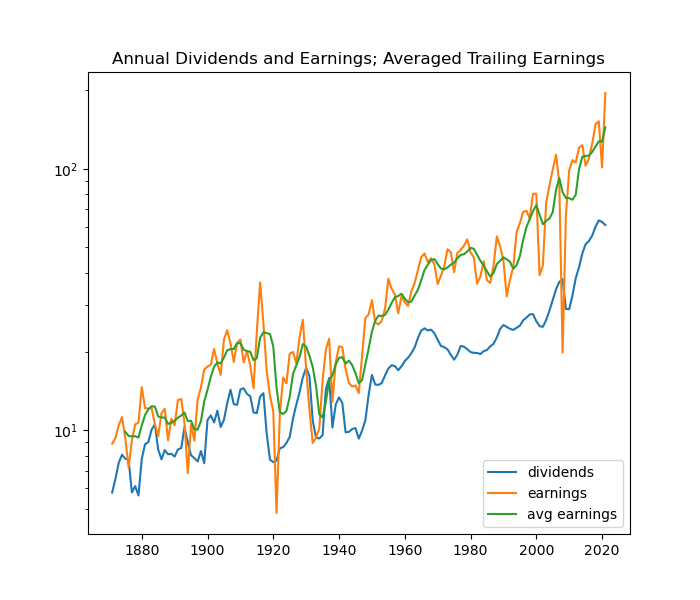
\includegraphics[width = 12cm]{combined.png}
\caption{Inflation-adjusted annual earnings and dividends 1871--2019}
\label{fig:combined}
\end{figure}

\subsection{Cyclically adjusted PE ratio} In practice, annual earnings are very volatile. For example, in 2008 S\&P 500 earnings plummeted due to housing crash, only to recover in the next year. Thus last year's earnings might not be a good representation of the market's earnings and dividends potential. 

To solve this problem, Robert Shiller averaged earnings (inflation-adjusted) over the previous 10 years, see \cite{Shiller1998}. For example, earnings averaged over 2010--2019 correspond to year 2019. These are called {\it 10-year trailing earnings}. The index level divided by these 10-year trailing earnings is called the {\it cyclically adjusted price-earnings ratio} (CAPE), or the {\it Shiller PE ratio}. It does a better job predicting next year's total inflation-adjusted returns than the standard PE ratio. Here, we do averaging over the previous 5 years instead of 10 years. This will still smooth out annual earnings, but will leave more data points for earnings: 147 instead of 142. See \textsc{Figure~\ref{fig:cape}}.

\subsection{Dividends and buybacks} Continuing the quote on \cite[pp.325--326]{RW12}:

\begin{quote}
Many analysts question whether dividends are as relevant now as they were in the past. They argue that firms increasingly prefer distributing their growing earnings to stockholders through stock repurchases rather than dividend payments. Two reasons are offered for such behavior --- one serves shareholders and the other management.
\end{quote}

Companies can distribute earnings to shareholders using buybacks instead of payouts, or reinvest them into business, which raises future earnings and dividends. Whether the {\it payout ratio} (fraction of earnings paid out as dividends) is an important indicator is a hotly debated topic, starting from the classic article \cite{MM61}, which gives a negative answer to this question. To capture their argument informally: Lower dividend yield now leads to more earnings reinvested into business and thus raise future earnings and dividend growth. See the survey \cite{DividendSurvey} for a comprehensive review of literature defending each side of this controversy. Recently, corporate payout and buyback policy was incorporated into the classic P/E research by Robert Shiller, see  \cite{Bunn, Farouk}. Thus we can view annual total real return minus annual real earnings growth as implied dividend yield. Arguably, this implied dividend yield is a more comprehensive measure than actual dividend yield. 

\subsection{The new bubble measure} As discussed earlier, wealth $V(t)$ (with reinvested dividends) growth in 1871--2022 is 6--7\% per year (after adjusting for inflation), but earnings $F(t)$ growth is 2\% per year. Taking logarithm and the difference, we have: $Q(t) = \ln V(t) - \ln F(t)$. This quantity grows at a linear rate (the difference between 6--7\% and 2\%). After detrending, we get a stationary time series: $H(t) = Q(t) - ct$. This is our new {\it bubble  measure.} We fit an autoregressive AR(1) for this time series:
$$
H(t) - h = b(H(t) - h) + \varepsilon(t),\quad \varepsilon(t) \sim \mathcal N(0, \sigma^2)\quad \mbox{i.i.d.} 
$$
The trend $c$ corresponds to average dividend yield, and the fluctuations around this trend correspond to the speculative return (valuation change). We explain three components of total return: two fundamental and one speculative. 

This is a different valuation measure than the CAPE or its logarithm. They give opposite results: The new measure indicates that currently (as of January 2022) the U.S. stock market is undervalued and future returns are higher than historical averages. The old measure indicates the opposite. 

In the classic Shiller CAPE, we compare only prices and earnings without regard to dividends. For the new bubble measure, we compare total returns with earnings growth only, and dividend yield is featured indirectly, through detrending. 

Recall that out of three return components: earnings growth, dividend yield, and changes in the P/E ratio, we labeled the first two {\it fundamental}, and the third one {\it speculative}. Now we merge the second and the third component in this implied dividend yield. To distinguish between its speculative and fundamental parts, we assume that this implied dividend yield fluctuates around the long-term average. In our research, we find that the intrinsic long-run average for this implied dividend yield is $c = 4.6\%$. 

However, in the short run it can deviate from this number. If it significantly exceeded this average for the last few years, then the market can be considered overheated and overpriced. Thus the bubble measure is the cumulative sum of all past annual implied dividend yields, minus true long-term average times the number of years elapsed. This detrending will be included into the regression. Thus we regress next year's implied dividend yield upon last year's detrended bubble measure.

\begin{figure}[t]
\subfloat[CAPE]{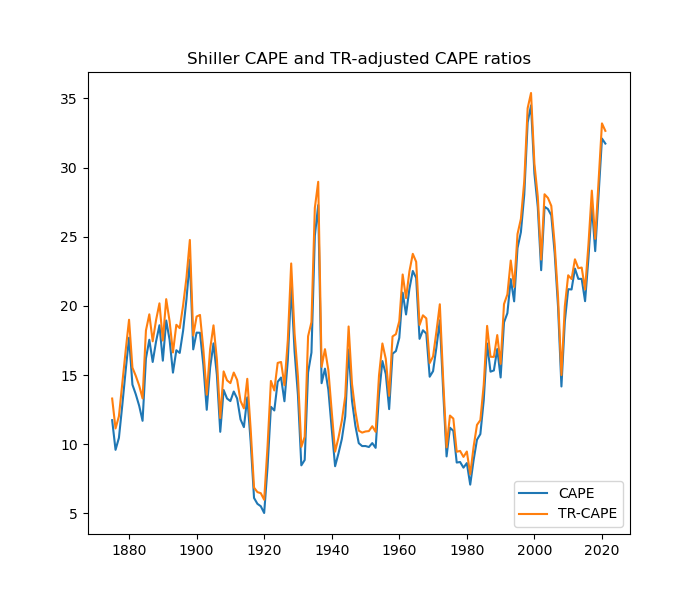
\includegraphics[width = 8cm]{CAPE-both.png}}
\subfloat[New bubble Measure]{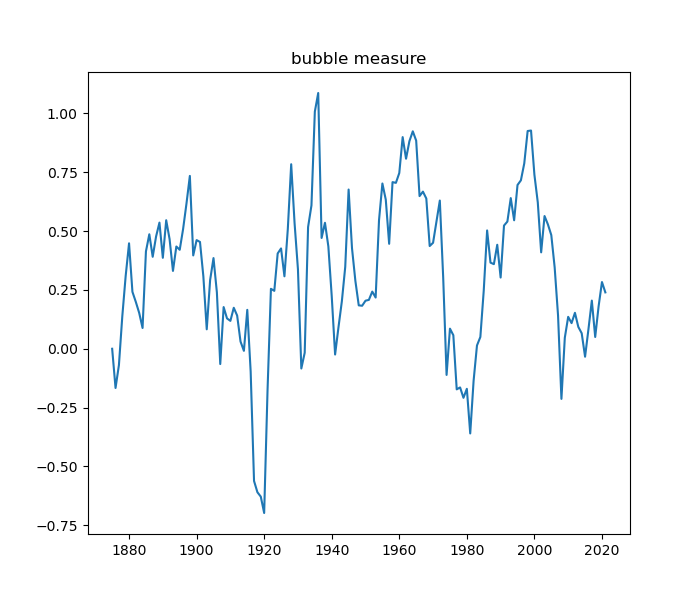
\includegraphics[width = 8cm]{bubble.png}}
\caption{CAPE, classic and TR-adjusted versions; and the new bubble measure}
\label{fig:cape}
\end{figure}

The difference between total returns and earnings growth fluctuates as AR(1) around its mean value, which is approximately 4--5\%. Consider a stagnant economy (with no population growth and no scientific-technological progress and thus no earnings growth). Then the total return fluctuates around 4--5\%. In his classic book, Thomas Piketty observes, see \cite[p.206]{Capital}:

\begin{quote}
\ldots traditional rate of conversion from capital to rent in the 18th and 19th centuries, for the most common and least risky forms of capital (typically land and public debt), was generally on the order of 5\%/year.
\end{quote}

In these agrarian societies, economic growth and therefore earnings growth was almost 0\%. To quote Piketty from \cite[p.353]{Capital}:

\begin{quote}
Economic growth was virtually nil throughout much of human history: cobining demographic and economic growth, we can say that the annual growth rate from antiquity to the 17th century never exceeded 0.1--0.2\%/year. Despite the many historical uncertainties, there is no doubt that the rate of return on capital was always considerably greater than this: the central value observed over the long run is 4--5\%/year. In particular, this was the return on land in most traditional agrarian societies. 
\end{quote}

Thus 4--5\%/year can be thought of as pure return on capital other than growth. The new bubble measure shows stability of this pure return fluctuating around this 4--5\% level. Only earnings growth is left as exogenous. Two other components: dividend yield and valuation changes are explained as AR(1). The new bubble measure describes two out of three components of total returns.

\subsection{Comparison of CAPE and the bubble measure} We plot two centralized valuation measures: logarithm of CAPE and the new bubble measure, in \textsc{Figure~\ref{fig:compare}}. As we see, two measures are very close in the 19th and 20th century, but sharply diverge in the 21st century. The CAPE shows that (as of January 2022) the market is overpriced, but the bubble measure shows the opposite. 


\begin{figure}[t]
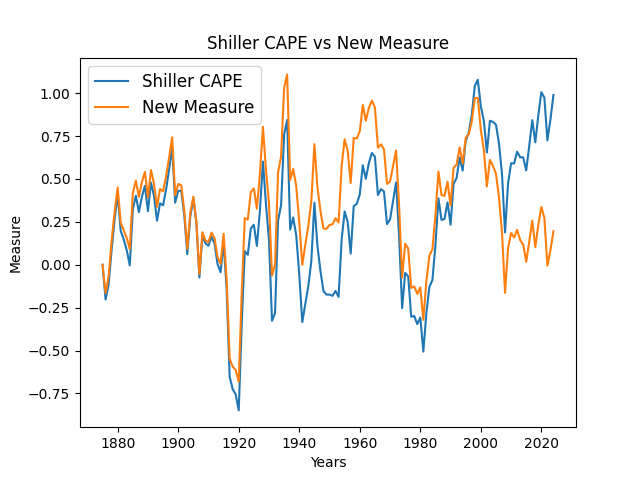
\includegraphics[width = 12cm]{compare.png}
\caption{Logarithm of CAPE (normalized to be zero in 1871) and bubble}
\label{fig:compare}
\end{figure}

\subsection{Adjustment of CAPE for dividends} In the articles \cite{Bunn, Farouk} we get the modification of CAPE version which Shiller called {\it total returns -- cyclically adjusted price-earnings ratio}, or TR-CAPE; see \textsc{Figure~\ref{fig:cape}}. This is computed as follows.

Investing 1\$ at the beginning of data in 1871 and reinvesting dividends, compute total wealth for each year. This wealth grows much faster than the index, as seen in \textsc{Figure~\ref{fig:index}.} Divide this wealth by the index level (adjusted so that 1871 = 1\$) and get the correction coefficient which measures, loosely speaking, wealth produced only by dividends, not by capital gains. We multiply each year's earnings by this correction coefficient. This gives us modified earnings.

Average them over the previous 5 years, and divide the wealth by these trailing 5-year modified earnings. We put wealth, not index level, in the numerator, to adjust it for dividends (or, equivalently, for total return) as well. Like the original Shiller CAPE ratio, we expect the TR-CAPE to fluctuate around a long-term average. If the CAPE or TR-CAPE exceeds its long-term average, we expect future returns to be lower. 

Recall our split of market returns into three components: two fundamental (earnings growth and dividend yield) and one speculative (change in valuation). Here we united two fundamental components into one (growth of 5-year trailing total return-adjusted earnings). Thus we can study our specuative component as a stock market valuation measure. 

This TR-CAPE measure theoretically seems better than the original Shiller CAPE. But, in practice, these measures are very close: see \textsc{Figure~\ref{fig:cape} (A).} The bubble measure is substantially different from Shiller CAPE; the TR-CAPE is not. Thus we shall not study this modified measure, since it is not an improvement over the classic 5-year CAPE.

\section{Statistical Analysis}

\subsection{Data and notation} We use annual data 1871--2022 in the spreadsheet \texttt{data7.xlsx} in our repository \texttt{asarantsev/IDY} on GitHub. One can find the data details in the \texttt{readme} sheet of this file. Our benchmark index is the Standard \& Poor 500, created in 1957, and its predecessors before this year. We take January daily close average data. Below, we simply refer to this index as {\it the index}. Robert Shiller's data also contains January Consumer Price Index (CPI) level, as well as annual earnings and dividends per share. We let $t = 1$ to be year 1871, and $t = 151$ to be year 2022. The total number of years is $T = 151$. By {\it start of year $t$} we mean January of year $t$. We denote by $d(t)$ and $e(t)$ nominal dividends and earnings for year $t = 1, \ldots, T$, by $s(t)$ the nominal value of the index in January (daily close average) of year $t+1$, for $t = 0, \ldots, T$. Finally, by $C(t)$ we denote the CPI in January of year $t+1$, for $t = 0, \ldots, T$. We adjust dividends, earnings, and the index for inflation:
$$
D(t) = \frac{C(T)}{C(t)}d(t),\quad E(t) = \frac{C(T)}{C(t)}e(t),\quad S(t) = \frac{C(T)}{C(t)}s(t).
$$
We will work only with {\it real} (inflation-adjusted) earnings, dividends, and the index.  For $S(t-1)$ invested in January of year $t$, we could buy 1 share of the index, which will cost $S(t)$ in January of year $t+1$, and will bring us dividend $D(t)$. Thus $S(t-1)$ invested in January of year $t$ turns into $S(t) + D(t)$ by January of year $t+1$. Total returns in year $t$ are:
$$
Q(t) = \ln\frac{S(t)+D(t)}{S(t-1)}.
$$
Here and below, we take logarithmic returns and growth. The wealth process is given by 
\begin{equation}
\label{eq:wealth}
V(t) = \exp(Q(1) + \ldots + Q(t)),\quad t = 0, \ldots, T.
\end{equation}
This is the total wealth (including reinvested dividends) for 1\$ invested in January 1871. The inflation-adjusted S\&P index and the wealth process are shown in \textsc{Figure}~\ref{fig:index}. 

\subsection{The main linear regression} To smooth out annual earnings fluctuations, consider averaged 5-year trailing inflation-adjusted earnings: 
$$
F(t) = \frac15(E(t) + \ldots + E(t-4)).
$$
The letter $F$ stands for {\it fundamental:} a valuation measure of stocks related to their actual eonomic activity, rather than market prices. Annual {\it real earnings growth} is
$$
G(t) = \ln\frac{F(t)}{F(t-1)}. 
$$
{\it Implied dividend yield} is equal to total real returns minus real earnings growth:
\begin{equation}
\label{eq:idy-def}
\Delta(t) = Q(t+5) - G(t+5),\quad t = 1, \ldots, 146.
\end{equation}
We fit the linear regression (assuming $\Delta(1) + \ldots + \Delta(t) = 0$ for $t = 0$), see \textsc{Table}~\ref{table:reg-results}:
\begin{equation}
\label{eq:main-reg}
\Delta(t+1) = \alpha + \beta t - \gamma(\Delta(1) + \ldots + \Delta(t)) + \varepsilon(t),\, t = 0, \ldots, 145.
\end{equation}
The $R^2 = 8\%$.

\begin{table}
\begin{tabular}{|c|c|c|c|}
\hline
coefficient & point estimate & $p$-value & [2.5\%, 97.5\%] CI \\
\hline
$\alpha$ & 0.0974 & 0.2\% & [0.035, 0.160] \\
\hline
$\beta$ & 0.0072 & 0.1\% & [0.003, 0.011] \\
\hline 
$\gamma$ & 0.1573 & 0.1\% & [0.069, 0.246] \\
\hline
\end{tabular}
\vspace{0.2cm}
\caption{Regression Results~\eqref{eq:main-reg}.}
\label{table:reg-results}
\end{table}

\subsection{Rewriting regression as autoregression}  Rewrite~\eqref{eq:main-reg} as a classic AR(1): 
\begin{equation}
\label{eq:bubble-ar1}
H(t+1) - h = b(H(t) - h) + \varepsilon(t),\quad H(t) = \Delta(1) + \ldots + \Delta(t) - ct. 
\end{equation}
Coefficients $b, c, h$ are to be determined. We can express using~\eqref{eq:bubble-ar1}:
\begin{equation}
\label{eq:idy}
\Delta(t+1) = H(t+1) - H(t) + c = (H(t+1) - h) - (H(t) - h) + c.
\end{equation}
Using~\eqref{eq:idy} to rewrite~\eqref{eq:bubble-ar1} and comparing  with~\eqref{eq:main-reg}, we get:
\begin{align}
\label{eq:alt-reg}
\begin{split}
\Delta(t+1) &= (b-1)(H(t) - h) + c + \varepsilon(t) \\ & = (b-1)(\Delta(1) + \ldots + \Delta(t) - ct - h) + c + \varepsilon(t).
\end{split}
\end{align}
Comparing coefficients in~\eqref{eq:main-reg} and~\eqref{eq:alt-reg}, we get: 
\begin{align}
\label{eq:new-coeff}
\begin{split}
b - 1 &= -\gamma;\quad -c(b - 1) = \beta;\quad -h(b-1) + c = \alpha;\quad \mbox{thus}\\
b &= 1 - \gamma;\quad c = \frac{\beta}{\gamma},\quad h = \frac{\alpha - c}{\gamma}.
\end{split}
\end{align}
Plugging point estimates for $\alpha, \beta, \gamma$ from \textsc{Table} 1 into~\eqref{eq:new-coeff}, we get:
\begin{equation}
\label{eq:new-est}
b = 0.84,\quad c = 4.6\%,\quad h = 0.33.
\end{equation}
These point estimates in~\eqref{eq:new-est} are important. Below, we discuss each of these parameters. 

\subsection{Economic meaning of the autoregression coefficients} The parameter $b$ is responsible for mean reversion: Since $b \in (0, 1)$, this  autoregression is indeed mean-reverting, not a random walk. As discussed, we reject the unit root hypothesis, which in this context means $b = \pm 1$. The closer $b$ to zero, the stronger the mean reversion is. 

The parameter $c$ is the long-run average of the implied dividend yield 
$\Delta$. This can be viewed as the long-term value of the second component of returns. As discussed earlier, this number matches the return on the capital in traditional societies with zero economic and earnings growth. 

Finally, $h$ is the long-term average of the bubble measure. Comparing the current bubble measure with $h$, one can find whether the stock market is over- or underpriced. The current (as of January 2022) value of $H$ is equal to $H(146) = 0.24 < h$. Thus the current stock market is underpriced, and future total real returns, given the same real earnings growth as in the last 151 years, are higher.

\subsection{Statistical analysis of real earnings growth}
We remark that white noise testing for real earnings growth terms $G(t)$ forces us to reject the hypotheses that this is white noise. The Shapiro-Wilk and Jarque-Bera testing also show that these terms are not Gaussian. See the autocorrelation and the quantile-quantile (vs Gaussian distribution) plots for real earnings growth time series in \textsc{Figure}~\ref{fig:growth}. 

Residuals $\varepsilon(t)$ are correlated with real earnings growth terms $G(t)$. The values of corelation coefficients are: $-28\%$ (Pearson), $-20\%$ (Spearman). Both of these are statistically significant, since the $p$-values are less than $5\%$ ($0.05\%$ for Pearson and $1.7\%$ for Spearman). We are interested in robust Spearman correlation, because the real earnings growth terms $G(t)$ are not Gaussian. 

The empirical mean of real earnings growth terms is 1.84\%, and the empirical standard deviation is 8.10\%. This is much lower than the empirical standard deviation of total real returns, which is 17\%. This implies we reduced variance by doing this regression analysis. This makes it valuable, even though we could not explicitly model real earnings growth time series. We sample real earnings growth using block bootstrap (see later in this article). 

\begin{figure}[t]
\subfloat{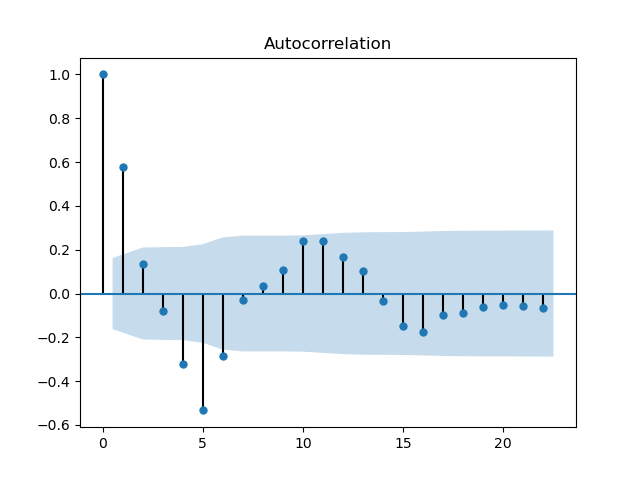
\includegraphics[width = 8cm]{acf-growth.png}}
\subfloat{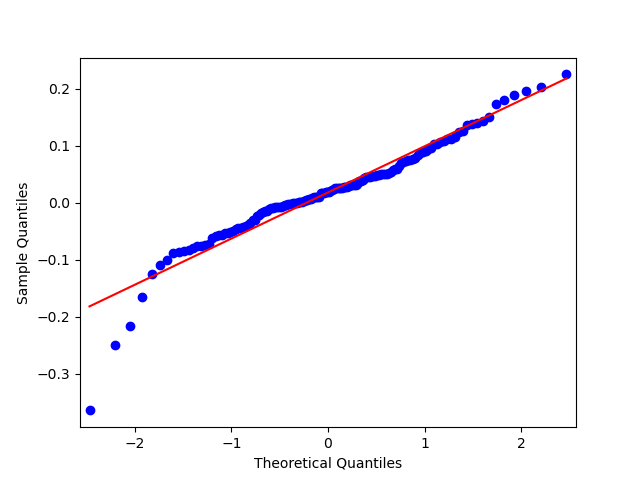
\includegraphics[width = 8cm]{qq-growth.png}}
\caption{Real earnings growth: autocorrelation and quantile-quantile plot}
\label{fig:growth}
\end{figure}


\subsection{Testing residuals for white noise and normality} The Ljung-Box white noise test for original values of residuals $\varepsilon(t)$ has $p = 9\%$ for lag 5 and $p = 10\%$ for lag 10; and for absolute values of residuals $|\varepsilon(t)|$ has $p = 9\%$ for lag 5 and $p = 17\%$ for lag 10. For each of these tests, we fail to reject the hypothesis that residuals form a white noise (with the classic significance level $5\%$). 

The results of Gaussian testing for residuals $\varepsilon(t)$ are as follows: $p = 39\%$ for Shapiro-Wilk and $p = 28\%$ for Jarque-Bera. The quantile-quantile plot for these residuals vs the Gaussian distribution is given in~\textsc{Figure}~\ref{fig:qq-res}. Thus we fail to reject the hypothesis that residuals are Gaussian, on the classic significance level $5\%$. The empirical standard deviation for these residuals is $\sigma = 18\%$. 

Based on the above, it is reasonable to assume that $\varepsilon(t) \sim \mathcal N(0, \sigma^2)$ are i.i.d. Gaussian. 

\subsection{Testing regression coefficients} Therefore, we can use Student $t$-test for each coefficient $\alpha, \beta, \gamma$. The $p$-values for this test are given in \textsc{Table}~\ref{table:reg-results}. They are much lower than the standard level 5\%. Thus all coefficients are significantly different from zero. Of particular importance is the coefficient $\beta$, which is responsible for mean reversion. 

The parameter $b$ is between $0$ and $1$. This implies that the autoregression~\eqref{eq:bubble-ar1} is mean-reverting, that is, has long-term stability. We could apply the stationarity or unit root testing for this time series $H(0), H(1), \ldots$ 

However, since residuals are i.i.d. Gaussian, we could use the aforementioned Student $t$-test for $\gamma$ as the unit root test: the 95\% confidence interval for $\gamma$ computed using the Student distribution lies wholly in $(0, 1)$; therefore, we reject the unit root hypothesis on the 95\% significance level. 

\begin{figure}[t]
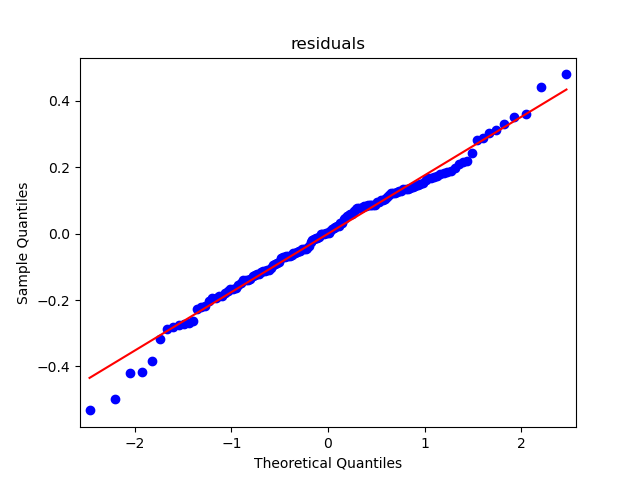
\includegraphics[width = 10cm]{qq-res.png}
\caption{Quantile-quantile plot: Regression residuals}
\label{fig:qq-res}
\end{figure}

\section{Model Statement and Theoretical Results} In this section, we create a time series model based on the statistical analysis in the previous section. We operate on a filtered probability space $(\Omega, \mathcal F, (\mathcal F_0, \mathcal F_1, \ldots), \mathbb P)$. We state the following well-known definitions from Stochastic Processes theory.

\begin{definition} A real-valued discrete-time stochastic process $X = (X_0, X_1, \ldots)$ is called {\it adapted} with respect to the given discrete-time filtration if $X_t$ is $\mathcal F_t$-measurable. The process $X$ has a {\it stationary distribution} $\pi$ if $X_t \sim \pi$ for all $t = 0, 1, 2, \ldots$
\label{defn:general}
\end{definition}

Gather equations from~\eqref{eq:idy} and~\eqref{eq:idy-def} and introduce the following concepts.

\begin{definition} Take a positive adapted stochastic process $F = (F(0), F(1), \ldots)$ which we call {\it fundamentals}. Take another adapted white noise sequence $\varepsilon(t) \sim \mathcal N(0, \sigma^2)$ for $t = 1, 2, \ldots$ Here, $\varepsilon(t)$ is independent of $\mathcal F_{t-1}$. Fix {\it average implied dividend yield} $c > 0$, {\it long-term bubble measure} $h$, and a {\it mean-reversion coefficient} $b \in (0, 1)$. {\it Total real returns} $Q(t)$ for year $t$ are defined as
\begin{equation}
\label{eq:model}
Q(t) = H(t) - H(t-1) + c + G(t),\, t = 1, 2, \ldots
\end{equation}
and {\it fundamental growth} $G(t)$ for year $t$ is defined by
\begin{equation}
\label{eq:growth-def}
G(t) = \ln\frac{F(t)}{F(t-1)},\, t = 1, 2, \ldots
\end{equation}
with {\it fundamental process} $F$, {\it average implied dividend yield} $c$, {\it bubble measure} $H$.  The latter is governed by the equation~\eqref{eq:bubble-ar1}. 
\label{defn:process}
\end{definition}

\begin{definition} {\it Average annual total real returns} for $T$ years are defined as 
\begin{equation}
\label{eq:def-avg}
\overline{Q}(T) = \frac1T\left[Q(1) + \ldots + Q(T)\right].
\end{equation}
{\it Real wealth} by year $T$ (starting from wealth $1$ at year $0$) from~\eqref{eq:wealth} is 
\begin{equation}
\label{eq:def-wealth}
V(T) = \exp(Q(1) + \ldots + Q(T)) = \exp(T\overline{Q}(T)).
\end{equation}
\label{defn:avg}
\end{definition}

We do {\it not} require $\varepsilon$ and $G$ to be independent or uncorrelated. Together, Definitions~\ref{defn:process} and~\ref{defn:avg} form a discrete-time model. This is the main model of this article. In the rest of this section, we analyze this model. For some of our theorems, we impose an additional assumption: strong mixing. This assumption does not specify a particular model for real earnings growth. 
%This implies the Strong Law of Large Numbers and the Central Limit Theorem.

\begin{asmp} The process $G$ is {\it stationary in the strong sense:} The distributions of $(G(1), \ldots, G(t))$ and $(G(s+1), \ldots, G(s + t))$ are the same for all $t, s = 1, 2, \ldots$ Next, $\mathbb E[G^2(t)] < \infty$. Finally, the process is {\it strong mixing:} There exists a sequence $(\alpha_n)_{n \ge 1}$ of positive numbers converging to $0$ such that for every $n, t, m = 1, 2, \ldots$, any Borel sets $B' \subseteq \mathbb R^{t}$ and $B'' \subseteq \mathbb R^m$, 
\begin{align}
\label{eq:mix}
\begin{split}
|\mathbb P&\left[\mathcal B' \cap \mathcal B''\right]  - \mathbb P(\mathcal B')\mathbb P(\mathcal B'')| \le \alpha_n;\\
\mathcal B' &:= \{(G(1), \ldots, G(t)) \in B'\},\\  \mathcal B'' & := \{(G(n+t+1), \ldots, G(n+m+t)) \in B''\}.
\end{split}
\end{align}
\label{asmp:strong-mixing}
\end{asmp}

Condition~\eqref{eq:mix} states that dependence between the first $t$ years and the years starting from $n+t$ (with the gap of $n$ years) decreases to zero as $n \to \infty$. This assumption seems reasonable: Earnings growth between 1881--1900 and 
between 2001--2021 seem independent or almost independent. This strong mixing assumption implies Strong Law of Large Numbers (SLLN), often called {\it ergodicity} in this context. However, we would also like to state Central Limit Theorem (CLT). Strong mixing is not quite enough for this result. We need stronger conditions. Many of them are available in \cite{ETBook}. We chose one below. 

\begin{asmp} Define $V_T := \mathrm{Var}(G(1) + \ldots + G(T))$ and assume $V_T \to \infty$ as $T \to \infty$. There exist constants $\delta, C > 0$ such that 
$$
\mathbb E\left[G(1) + \ldots + G(T)\right]^{2(1+\delta)} \le CV^{1 + \delta}_T,\quad T = 1, 2, \ldots
$$
\label{asmp:CLT}
\end{asmp}

Next, we state a Markovian assumption: that real earnings growth term $G(t)$ for time $t$ depends not on the entire history $G(1), \ldots, G(t-1)$ and $\varepsilon(1), \ldots, \varepsilon(t)$, but instead only on $G(t-1)$ and $\varepsilon(t)$. Without loss of generality, we assume that $G(0)$ also exists and is an $\mathcal F_0$-measurable random variable. 

\begin{asmp}
There exists a {\it transition density} $\mathbf{p} : \mathbb R^3 \to (0, \infty)$: a  function which is continuous in $(x, y)$, such that for every $A \subseteq \mathbb R$, we have: 
$$
\mathbb P(G(t) \in A\mid G(t-1) = x, \varepsilon(t) = y) = \int_A\mathbf{p}(x, y, z)\mathrm{d}z.
$$
\label{asmp:Markov}
\end{asmp}

Finally, we state a moment boundedness assumption for $G$ and $H$, in case $G$ is not in its stationary version. 

\begin{asmp} $\sup_{t \ge 0}\mathbb E[G^{p}(t)] < \infty$ and $\mathbb E[H(0)|^p < \infty$ for some $p > 1$. 
\label{asmp:bdd}
\end{asmp}

Below are main results. The proofs are in the Appendix. First, a technical lemma.

\begin{lemma} Average annual total real returns for $T$ years are given by
\begin{equation}
\label{eq:mean-return}
\overline{Q}(T) = c + \frac{H(T) - H(0)}T + \overline{G}(T),
\end{equation}
and wealth at time $T$ is given by 
\begin{equation}
\label{eq:total-wealth}
V(T) = \exp\left[cT + H(T) - H(0)\right]\frac{F(T)}{F(0)}.
\end{equation}
\label{lemma:main}
\end{lemma}

Our next result is the Strong Law of Large Numbers (SLLN) for total real returns. It follows from Assumption of the SLLN for real earnings growth, as well as mean reversion of the autoregressive process.

\begin{theorem} Under Assumption~\ref{asmp:strong-mixing}, we have the following asymptotic results: as $T \to \infty$, 
\begin{align}
\label{eq:limiting-delta}
\frac1T(\Delta(1) + \ldots + \Delta(T)) \to c\quad \mbox{almost surely.}
\end{align}
Average total real returns satisfy the convergence statement:
\begin{equation}
\label{eq:R-LLN}
\overline{Q}(T) \to c + g\quad \mbox{almost surely as}\quad T \to \infty.
\end{equation}
\label{thm:SLLN}
\end{theorem}

Further, we state ergodicity (long-term stability) result for the process $(G, H)$. For probability measures $P$ and $Q$ on $\mathbb R^2$, define the {\it total variation distance}: 
\begin{equation}
\label{eq:TV}
d_{\mathrm{TV}}(P, Q) = \sup\limits_{A \subseteq \mathbb R^2}|P(A) - Q(A)|,
\end{equation}
and the {\it Wasserstein distance of order} $p \ge 1$: 
\begin{equation}
\label{eq:W-p}
\mathcal W_p(P, Q) = \inf\limits_{X \sim P, \, Y \sim Q}\left[\mathbb E|X - Y|^p\right]^{1/p}.
\end{equation}
In~\eqref{eq:W-p}, the inf is taken over all {\it couplings:} pairs of random variables $(X, Y)$ such that $X \sim P$ and $Y \sim Q$. Both these functions are indeed distances:~\eqref{eq:TV} is on the set $\mathcal P$ of all probability measures on $\mathbb R^2$, and~\eqref{eq:W-p} is on the set of all $P \in \mathcal P_2$ with finite $p$th moment. A discrete-time Markov process $X = (X(0), X(1), \ldots)$ on the state space $\mathbb R^2$ has a {\it stationary distribution} $\Pi$ (a probability measure on $\mathbb R^2$) if $X(0) \sim \Pi$ implies $X(1) \sim \Pi$ (hence $X(t) \sim \Pi$ for all $t$).

\begin{theorem}
\label{thm:Markov}
Under Assumption~\ref{asmp:Markov}, the process $(G, H)$ is Markov, time-homogeneous. 
\end{theorem}

\begin{theorem}
\label{thm:ergodic}
Under Assumption~\ref{asmp:Markov} and~\ref{asmp:bdd}, 

(a) the process $(G, H)$ has a unique stationary distribution $\Pi$ on $\mathbb R^2$ with positive Lebesgue density on $\mathbb R^2$, with finite $p$th moments, and a Gaussian marginal for $H$: $\Pi_H = \mathcal N(h, \sigma^2_{\Pi})$, where 
$\sigma^2_{\Pi} = \sigma^2/(1 - b^2)$;

(b) regardless of the initial distribution, the distribution of $(G(t), H(t))$ converges to $\Pi$ as $t \to \infty$ in the total variation and in the Wasserstein distance of order $p$.  
\end{theorem}

Finally, we state the CLT for total real returns: In the long run, wealth is a lognormal random variable. This follows from the CLT assumption for the real earnings growth series. 

\begin{theorem}
Under Assumptions~\ref{asmp:strong-mixing}, ~\ref{asmp:CLT}, we have weak convergence
$$
\frac{Q(1) + \ldots + Q(T) - (c + g)T}{\sqrt{V_T}} \to \mathcal N(0, 1),\quad T \to \infty.
$$
\label{thm:CLT}
\end{theorem}


\begin{figure}[t]
\subfloat[$\varepsilon(t)$]{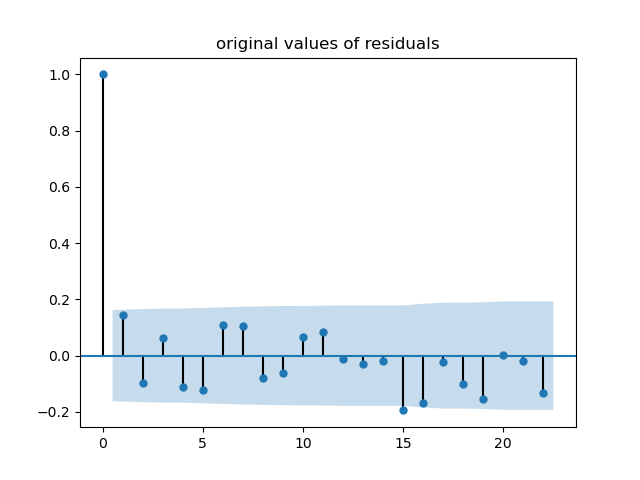
\includegraphics[width = 8cm]{acf-res.png}}
\subfloat[$|\varepsilon(t)|$]{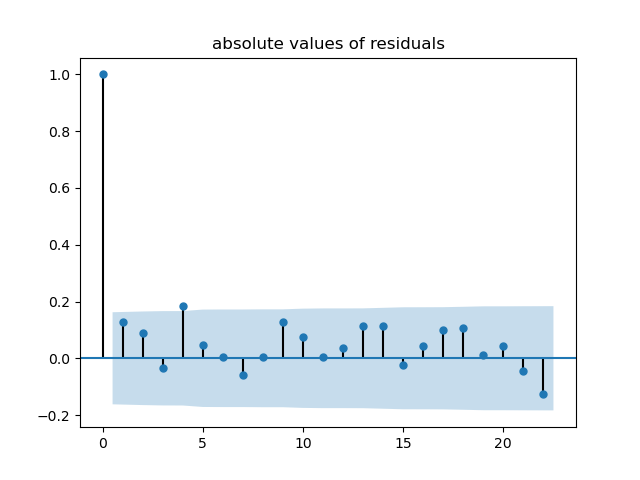
\includegraphics[width = 8cm]{acf-abs.png}}
\caption{ACF for original and absolute values of residuals $\varepsilon(t)$}
\label{fig:acf-bubble}
\end{figure}

\section{Equity-Linked Annuities and Withdrawal Rates} 



\subsection{Sustainable withdrawal processes} First, we consider rule (b), generalized for the case of changing (and possibly random) proportional withdrawal rate. 

\begin{definition} A {\it withdrawal process} $W = (W(0), W(1), \ldots)$ is a discrete-time stochastic process with values in $(0, 1)$. Its corresponding  {\it wealth process} is defined as
$$
V(t) = V(t-1)e^{G(t)+\Delta(t)}(1 - W(t)),\, t = 1, 2, \ldots;\quad V(0) = 1.
$$
\end{definition}

For example, if total real return $Q(t) = 7\%$, and withdrawal rate $W(t) = 4\%$, then wealth from $t-1$ to $t$ is multiplied by $e^{0.07}$ from total real return and is multiplied by $0.96$ from withdrawal. Thus the overall multiplication factor is $e^{0.07}\cdot 0.96 \approx 1.03$. If withdrawal process is not constant, we define an asymptotic rate: a long-term limit.

\begin{definition} A withdrawal process $W$ has {\it asymptotic rate} $w$ if it satisfies
$$
\frac1T\sum\limits_{t=1}^TW(t) \to w\quad \mbox{a.s. as}\quad T \to \infty.
$$
\end{definition}

For any withdrawal process, $V(t) > 0$ almost surely for all $t$. But still, $V(t)$ could decrease to small values, which is, of course, undesirable. We define a condition under which this does not happen. 

\begin{definition}
A withdrawal process is called {\it sustainable} if $V(t) \to \infty$ a.s. as $t \to \infty$. 
\end{definition}

Our main result is as follows: We prove sufficient conditions for sustainability, and other sufficient conditions for non-sustainability. There is a gap between these two results, because $c + g > 1 - e^{-c-g}$, so these are not necessary and sufficient conditions. To close this gap is left for future research. 

\begin{theorem} Under  Assumption~\ref{asmp:strong-mixing}, 

(a) any constant withdrawal process $W(t) = w < 1 - e^{-c-g}$ is sustainable;

(b) any withdrawal process with asymptotic rate $w > c + g$ is not sustainable.
\label{thm:withdrawal}
\end{theorem}


\subsection{Constant real withdrawal amounts} Now, let us switch to rule (a). Assume constant (adjusting for inflation) annual withdrawal rates $w$, the ruin (wealth less than zero) can happen. Real earnings growth was not modeled as i.i.d. or any other particular time series model. Therefore, it is hard to compute the ruin probability explicitly. However, we can use block bootstrap: choose a random block of $T$ years of real earnings growth terms between 1876 and 2021. For simplicity, we assume there is no correlation between real earnings growth terms and Gaussian residuals. This is not consistent with the data, but we use this assumption as useful but imperfect approximation. The simulation procedure is as follows.

\begin{enumerate}
\item Fix the initial bubble measure $H(0)$.

\item For $t = 1, \ldots, T$, simulate $H(t)$ using AR(1) with Gaussian noise $\varepsilon(t)$. 

\item Independently of $\varepsilon$, choose a $T$-year consecutive period in $1876, \ldots, 2021$ randomly (uniformly). Take earnings growth data $G(t)$ for $t$ in this period. 

\item Total returns $Q(t)$ for year $t$ is given by~\eqref{eq:model}.

\item Compute recursively wealth $V_w(t)$ at time $t$ using wealth $V_w(t-1)$ at time $t-1$: $V_w(t) = V_w(t-1)e^{Q(t)} - w$. 

\item Repeat steps 2-5 a given number of times. 

\item If at some step $t$ we get: $V_w(t) < 0$, we stop this simulation and consider this to be bankruptcy (ruin). Then we compute empirical ruin probability. 
\end{enumerate}

Take $T = 40$, which seems a reasonable retirement horizon. We invest in the stock market, reinvest dividends, and withdraw $w$ each year. We study two scenarios: (a) starting from the current (as of January 2022) bubble measure $x$; (b) starting from the long-term average bubble measure $h$. 

\begin{table}
\begin{tabular}{|c||c|c|c||}
\hline
\hline
Withdrawal Rate & 3\% & 4\% & 5\& \\
\hline
\hline
Current Bubble Measure & 0.1\% & 3\% & 13\% \\
\hline 
Average Bubble Measure & 0.3\% & 5\% & 18\% \\
\hline
\hline
\end{tabular}
\bigskip
\caption{Default probabilities. Results of 1000 simulations, 40 years.}
\end{table}

Thus 3\% and even 4\% withdrawal rate is relatively safe, in both scenarios. But 5\% withdrawal rate is not quite safe anymore: 10--20\% ruin probability is large.  Since $x < h$, ruin probabilities for starting with the current bubble measure $x$ are smaller than that for the average bubble measure $h$. 

%Let us compare these ruin probabilities with Standard \& Poor default rates for corporate bonds: 0.6\% for AAA, 1.5\% for AA, 2.91\% for A, and 10.29\% for BBB (the lowest investment-grade ranking).


\section{Discussion} 

In each two choices of valuation measure $M(t)$: classic CAPE and bubble; for each choice of averaging window $W$, we get the following decomposition of total returns:
\begin{equation}
\label{eq:decomp}
R(t) = \triangle M(t) + \Gamma(t) + \Delta(t),
\end{equation}
where $\Gamma$ is earnings growth rate for trailing 5-year averaged real earnings; $M$ is governed by an AR(1), with $\triangle M(t) \equiv M(t) - M(t-1)$; and $\Delta(t) = \ln(1 + D(t)/S(t))$ is the logarithmic dividend yield for classic CAPE, and $\Delta(t) = 0$ for the two other measures. Recall the three components of total returns: earnings growth, dividend yield, and valuation changes. We distribute them between terms in the right-hand side of~\eqref{eq:decomp} as follows:

(a) For the classic CAPE, $\triangle M$ is the valuation change, $\Gamma$ is earnings growth, and $\Delta$ is dividend yield.

(b) For the bubble measure, $\triangle M$ contains both change in valuation and dividend yield, and $\Gamma$ is earnings growth.


The original CAPE does not explain stock market returns without an additional term (depending on dividend yield). The two modifications of this model do explan stock market returns as the sum of an AR(1) process and earnings growth. 

Before 1920, annual real earnings growth was 1--2\% while dividend yield was 5\%. After 1970, annual real earnings growth is 4--5\%, dividend yield is 2\%. The dividend yield is chosen by corporate payout policies. If a company chooses to pay much of its earnings as dividends, then dividend yield is large, but retained earnings (used to pay debt, invest in expansion or R\&D, and make stock buybacks) are small; thus earnings growth must be smaller. Conversely, if a company chooses to buy back stock instead of paying dividends, then earnings per share increase faster. Thus actual earnings growth might differ from what one could call fundamental earnings growth, which is growth with non-changing dividend payout/stock buyback policy. Similarly, actual dividend yield might not be representative of fundamental dividend yield. Recall the Modigliani-Miller theorem that states indifference of total returns to dividend policy. 

We also discussed withdrawal strategies. More precisely, we tested whether the classic 4\% withdrawal rate (withdrawing 4\% of initial wealth, inflation-adjusted) is sustainable. The answer is affirmative. Even 5\% is still quite safe. But 6\% is no longer safe. 

As of January 2022, is the market over- or underpriced? The CAPE shows it is overpriced, but curret bubble is lower than its long-term average. In \textsc{Figure~\ref{fig:compare}}, we plot these two valuation measures: logarithm of CAPE and the bubble measure. Both are centralized by subtracting their historical averages. We can see that these two measures are very close until the start of the 21st century, but sharply diverge later. This can be attributed to recent reluctance of companies to pay dividends, as discussed in Section 2. This change was rather recent (last 20 years). If this aversion to dividends persists for another century, then CAPE might become elevated and no longer representative of the market conditions. Then the bubble measure will have stronger predictive power of future returns. 

Future research might be focused on modeling earnings growth. This will include economic forecasts, since corporate earnings are closely tied to overall economy and tax policy. In addition, a more detailed investigation for withdrawal rates is needed. Alternatively, one can replicate this research for individual stocks and stock portfolios, rather than the overall stock market index. Also, one can alleviate deficiency in our simulation study to include correlation between autoregression residuals and real earnings growth terms. 

Finally, we can include interest rates in our modeling (short-term Treasury bills, long-term Treasury bonds, and long-term AAA corporate rates), which are also available from 1871 onward. We can use these bond yields in our regression models.  Low bond yields make them less attractive and push stock prices upward, making CAPE higher. Since now we have historically low yields in the USA, this can explain historically high CAPE ratios. In addition, we can make portfolios of stocks (measured by the S\&P index) and bonds (Treasury or AAA corporate bonds). 

\section{Appendix}

\subsection{Proof of Lemma~\ref{lemma:main}} Equation~\eqref{eq:mean-return} follows from~\eqref{eq:def-avg} and the following computations:
\begin{align*}
\overline{Q}(T) & = \frac1{T}\left(\Delta(1) + \ldots + \Delta(T) + G(1) + \ldots + G(T)\right) \\ & = \frac1{T}\left(H(1) - H(0) + c + H(2) - H(1) + c + \ldots + H(T) - H(T-1) + c\right) \\ & + \frac1{T}\left(G(1) + G(2) + \ldots + G(T)\right) \\ & = c + \frac{H(T)}{T} - \frac{H(0)}{T} + \frac1{T}\left(G(1) + G(2) + \ldots + G(T)\right).
\end{align*}
Equation~\eqref{eq:total-wealth} follows from~\eqref{eq:growth-def} and~\eqref{eq:mean-return}.

\subsection{Proof of Theorem~\ref{thm:SLLN}} Let us prove~\eqref{eq:limiting-delta}. We can rewrite 
$$
\frac1T\left(\Delta(1) + \ldots + \Delta(T)\right) = \frac1T\left(cT + H(T) - H(0)\right) = c + \frac{H(T) - H(0)}T.
$$
Let us show that $H(T)/T \to 0$ a.s. Taking the expectation in~\eqref{eq:ar-initial}, we get: $\mathbb E[H(t)] - h = b(\mathbb E[H(t-1)] - h)$. Solving this recurrent relation, we get that the sequence $\mathbb E H(t),\, t = 0, 1, \ldots$ is bounded. Next, from~\eqref{eq:ar-initial}, $\mathrm{Var}(H(t)) = b^2\cdot\mathrm{Var}(H(t-1)) + \sigma^2$. Since $0 < b < 1$, we have: 
\begin{equation}
\label{eq:bdd-var}
\mathrm{Var}(H(t)) \le \frac{\sigma^2}{1 - b^2}. 
\end{equation}
Combining boundedness of expectation with~\eqref{eq:bdd-var}, we get: $\mathbb E\left[H^2(t)\right] \le C$ for all $t \ge 0$ and some constant $C$. By the Markov inequality, for every $a > 0$ we have: $\mathbb P(t^{-1}|H(t)| \ge a) \le \mathbb E\left[H^2(t)\right]/a^2t^2 \le C/a^2t^2$. From the Borel-Cantelli lemma, a.s. only finitely many events occur:
$\{t^{-1}|H(t)| \ge a\}$. Since this is true for all $a > 0$, we conclude that 
\begin{equation}
\label{eq:LLN-H}
t^{-1}H(t) \to 0\quad \mbox{a.s. as}\quad t \to \infty.
\end{equation}
By \cite[Section 28.5, Theorem 6]{FGBook}, from Assumption~\ref{asmp:strong-mixing}, we have Strong Law of Large Numbers for the process $G$: almost surely, 
\begin{equation}
\label{eq:LLN-G}
\frac{G(0) + \ldots + G(T-1)}{T} \to g := \mathbb E[G(1)],\quad T \to \infty.
\end{equation}
Combining~\eqref{eq:LLN-H} with~\eqref{eq:LLN-G}, we complete the proof of Theorem~\ref{thm:SLLN}.

\subsection{Proof of Theorem~\ref{thm:Markov}} Define the density of $\mathcal N(0, \sigma^2)$: $\varphi(z) = [\sqrt{2\pi}\sigma]^{-1}\exp\left[-z^2/2\sigma^2\right]$. Then we can express $\varepsilon(t) = H(t) - h - b(H(t-1) - h)$ using~\eqref{eq:bubble-ar1}. Therefore, the transition density of $(G, H)$: condition density of $(G(t), H(t))$ at $(g_1, h_1)$ given $G(t-1) = g_0$ and $H(t-1) = h_0$, is given by
\begin{equation}
\label{eq:transition}
\mathbf{p}(g_0, h_1 - h - b(h_0 - h), g_1)\varphi(h_1 - h - b(h_0 - h)).
\end{equation}

\subsection{Proof of Theorem~\ref{thm:ergodic}} {\it Step 1.} The function $\mathbf{p}$ from Assumption~\ref{asmp:Markov} is strictly positive for any argument values. The Gaussian density is strictly positive too. Thus, the same is true for the function~\eqref{eq:transition}. Therefore, the Markov process $(G, H)$ has the {\it positivity property:} For a subset $A \subseteq \mathbb R^2$ of positive Lebesgue measure, and for any $g_0, h_0 \in \mathbb R^2$, 
\begin{equation}
\label{eq:pve}
\mathbb P((G(1), H(1)) \in A\mid G(0) = g_0,\, H(0) = h_0) > 0.
\end{equation}

{\it Step 2.} Solve the recurrent equation~\eqref{eq:bubble-ar1}: $H(t) - h = b^{t-1}\varepsilon(1) + \ldots + \varepsilon(t) + b^t(H(0) - h)$. This random variable has the same distribution as $H'(t) = \sum_{s=1}^tb^{s-1}\varepsilon(s) + b^t(H(0) - h) + h$. The following series converges in $L^p$:
\begin{equation}
\label{eq:L-p}
H'(\infty) := \sum\limits_{s=1}^{\infty}b^{s-1}\varepsilon(s).
\end{equation}
Indeed, the $p$-norm of $\varepsilon(s)$ is constant (does not depend on $s$), and $b \in (0, 1)$. Therefore, the series~\eqref{eq:L-p} converges in $L^p$. We apply that the space $L^p$ is {\it Banach}, that is, every fundamental sequence converges.
Thus the sequence $H'(t) \to H'(\infty) + h$ as $t \to \infty$ in $L^p$. Therefore, the distribution of $H(t)$ (the same as that of $H'(t)$) converges in law to the distribution of $H'(\infty) + h$. In addition, the $p$th moments of $H(t)$ converges to the $p$th moment of $H'(\infty) + h$ as $t \to \infty$. Since convergence in $\mathcal W_p$ is equivalent to weak convergence plus convergence of $p$th moments, the above results implies convergence in $\mathcal W_p$. Finite $p$th moments of the stationary distribution $\Pi$ are implied by~\eqref{eq:bdd-g-h} and Fatou's lemma. We get the marginal distribution of $\Pi$ for $H$ from the observation that $H$ is an AR(1) with Gaussian innovations; see any classic text on time series, for example \cite{BrockwellDavis}. 

{\it Step 3.} Finally, let us show uniqueness of the stationary distribution and convergence in total variation. This follows from the two observations. First, as mentioned above, the process $(G, H)$ has the positivity property~\eqref{eq:pve}. Second, we have:
\begin{equation}
\label{eq:bdd-g-h}
\sup_t\mathbb E\left[|G(t)|^p + |H(t)|^p\right] < \infty.
\end{equation}
For $G$, this is in Assumption~\ref{asmp:bdd}; and for $H$, this was shown above, since $H'(t)$ converges in $L^p$ as $t \to \infty$. From~\eqref{eq:bdd-g-h}, we get that the sequence $(G(t), H(t))$ is {\it tight:}
\begin{equation}
\label{eq:tight}
\sup\limits_{t = 0, 1, \ldots}\left[\mathbb P(|G(t)| > u) + \mathbb P(|H(t)| > u)\right] \to 0,\quad u \to \infty.
\end{equation}
In \cite{MT1992}, the property~\eqref{eq:tight} is called {\it boundedness in probability}. This process $(G, H)$ is also irreducible (that is, it does not have two or more disconnected components of the state space $\mathbb R^2$), since the transition density is strictly positive everywhere. The function $\varphi$ from~\eqref{eq:Gauss} is contnuous. The function $\mathbf{p}$ from Assumption~\ref{asmp:Markov} is continuous in the first two arguments. Therefore, the Markov process $(G, H)$ is a {\it $T$-chain} in the sense of \cite[p.548]{MT1992}. Applying Corollary (ii) in \cite[p.550]{MT1992}, we conclude that the Markov process $H$ is {\it positive Harris recurrent} in the sense of \cite{MT1992}. Therefore, it has a unique stationary distribution. Applying \cite[Theorem 3.4]{MT1992} to Lebesgue measure $\psi$ (since $(G, H)$ is irreducible with respect to this Lebesgue measure), we get: all compact sets are petite. Apply \cite[Theorem 5.2(iii)]{MT1992}. Use the aperiodicity ($m = 1$ in the notation on the cited theorem), which follows from positivity of the transition density. This completes the proof of Step 3. 

\subsection{Proof of Theorem~\ref{thm:CLT}} We rewrite
\begin{align*}
&\frac{Q(1) + \ldots + Q(T) - (c+g)T}{\sqrt{V_T}} \\ & = \frac{G(1) + \ldots + G(T) - gT}{\sqrt{V_T}} + \frac{H(T) - H(0)}{\sqrt{V_T}}.
\end{align*}
By \cite{ETBook}, Assumption~\ref{asmp:CLT} implies the following Central Limit Theorem: 
$$
\frac{G(1) + \ldots + G(T) - gT}{\sqrt{V_T}} \Rightarrow \mathcal N(0, 1),\quad T\ \to \infty.
$$
It suffices to prove convergence in distribution (or in probability, which is equivalent):
$(H(T) - H(0))/\sqrt{V_T} \to 0$ as $T \to \infty$. In turn, it suffices to show convergence in $L^2$, which is stronger than convergence in probability. But this convergence follows from boundedness of the second moment of $H(t)$, shown during the proof of Theorem~\ref{thm:SLLN}. 

\subsection{Proof of Theorem~\ref{thm:withdrawal}} (a) We can rewrite $V(t) = V(t-1)e^{G(t)+\Delta(t) - w^*}$ for $t = 1, 2, \ldots$, where $w^* = -\ln(1 - w) < g + c$. By induction, $V(t) = \exp\left[G(1)+\ldots + G(t) + \Delta(1) + \ldots + \Delta(t) - tw^*\right]$. We can represent this exponent as $\ln V(t) = G(1) + \ldots + G(t) + H(t) - H(0) + ct - w^*t$. Using an earlier result~\eqref{eq:LLN-H}, we get:
$$
\frac1t\ln V(t) = \frac1t\sum\limits_{k=1}^tG(k) + \frac1tH(t) - \frac1tH(0) + c - w^* \to g + c - w^* > 0.
$$
Thus $V(t) \to \infty$ a.s. as $t \to \infty$. 

(b) Similarly,  $\ln V(t) = G(1) + \ldots + G(t) + H(t) - H(0) + ct + \ln(1 - W(1)) + \ldots + \ln(1 - W(t))$. Note that $-\ln(1 - w) \ge w$ for $w \in (0, 1)$. Thus $\ln V(t) \le G(1) + \ldots + G(t) + H(t) - H(0) + ct - W(1) - \ldots - W(t)$. Dividing by $t$ and letting $t \to \infty$, we have: 
$$
\frac1t\ln V(t) \le \frac1t\sum\limits_{k=1}^tG(k) + \frac{H(t)}t - \frac{H(0)}t + c  \to g + c - w < 0.
$$
Thus $\varlimsup\limits_{t \to \infty} V(t) \le 1$, and this withdrawal rate is not sustainable. 



%\section*{Declarations} 
%
%\subsection{Conflict of interest} The author does not have any conflict of interest.
%
%\subsection{Funding} The author did not receive any external funding for this research.
%
%\subsection{Availability of data and material} See the spreadsheet \texttt{data7.xlsx} in the \texttt{GitHub} repository \texttt{asarantsev/IDY}
%
%\subsection{Code availability} See the Python code \texttt{code.py} in the \texttt{GitHub} repository \texttt{asarantsev/IDY} 

\begin{thebibliography}{99}

\bibitem{Arnott} \textsc{Robert D. Arnott, Denis B. Chaves, Tzee-man Chow} (2017). King of the Mountain: The Shiller P/E and Macroeconomic Conditions. \textit{The Journal of Portfolio Management} \textbf{44} (1), 55--68.

\bibitem{Anna} \textsc{Anna R. Bacinello} (2014). Equity-Linked Life Insurance. In \textit{Wiley Statistics Reference Online}.

\bibitem{Guarantees} \textsc{Anna R. Bacinello, Fulvio Ortu} (1993). Pricing Equity-Linked Life Insurance with Endogenous Minimum Guarantees. \textit{Insurance: Mathematics and Economics} \textbf{12} (3), 245--257. 

\bibitem{DividendSurvey} \textsc{H. Kent Baker, Robert A. Weigand} (2015). Corporate Dividend Policy Revisited. \textit{Managerial Finance} \textbf{41} (2), 126--144. 

\bibitem{JPMorgan} \textsc{Alicia Barrett, Peter Rappoport} (2011). Price-Earnings Investing. \textit{JP Morgan Asset Management, Reality in Returns} \textbf{November 2011} (1), 1--12.

\bibitem{ActuarialBook} \textsc{Mathieu Boudreault, Jean-Francois Renaud} (2019). \textit{Actuarial Finance: Derivatives, Quantitative Models and Risk Management.} Wiley. 

\bibitem{IndexedAnnuity} \textsc{Phelim Boyle, Weidong Tian} (2008). The Design of Equity-Indexed Annuities. \textit{Insurance: Mathematics and Economics.} \textbf{43} (3), 303--315. 

\bibitem{BrockwellDavis} \textsc{Peter J. Brockwell, Richard A. Davis} (2016). \textit{Introduction to Time Series and Forecasting.} 3rd edition, Springer.

\bibitem{Bunn} \textsc{Oliver D. Bunn, Robert J. Shiller} (2014). Changing Times, Changing Values: A Historical Analysis of Sectors within the US Stock Market 1872--2013. NBER Working Paper 20370.

\bibitem{Shiller1998} \textsc{John Y. Campbell, Robert J. Shiller} (1998). Valuation Ratios and the Long-Run Stock Market Outlook. \textit{The Journal of Portfolio Management} \textbf{24} (2), 11--26.

\bibitem{ETBook} \textsc{Ernst Eberlein, Murad Taqqu} (1986). \textit{Dependence in Probability and Statistics: A Survey of Recent Results.} Birkhauser. 

\bibitem{FF1993} \textsc{Eugene F. Fama, Kenneth R. French} (1993). Common Risk Factors in the Returns on Stocks and Bonds. \textit{J. Fin. Econ.} \textbf{33} (1), 3--56.

\bibitem{FengBook} \textsc{Runhuan Feng} (2017). \textit{An Introduction to Computational Risk Managementof Equity-Linked Insurance.} CRC Press.

\bibitem{FGBook} \textsc{Bert E. Fristedt, Lawrence F. Gray} (1997). \textit{A Modern Approach to Probability Theory.} Springer.

\bibitem{Farouk} \textsc{Farouk Jivrai, Robert J. Shiller} (2017). The Many Colours of CAPE. Yale ICF Working Paper No. 2018-22.

\bibitem{RW12} \textsc{Burton Malkiel} (2019). \textit{A Random Walk Down Wall Street.} 12th edition, W. W. Norton \& Company.

\bibitem{MT1992} \textsc{Sean P. Meyn, Richard L. Tweedie} (1992). Stability of Markovian Processes I: Criteria for Discrete-Time Chains. \textit{Advances in Applied Probability} \textbf{24}, 542--575. 

\bibitem{MM61} \textsc{Merton H. Miller, Franco Modigliani} (1961). Dividend Policy, Growth, and the Valuation of Shares. \textit{The Journal of Business} \textbf{34} (4), 41--433. 

\bibitem{Acct} \textsc{Jane A. Ou, Stephen H. Penman} (1989). Accounting Measurement, Price-Earnings Ratio, and the Information Content of Security Prices. \textit{Journal of Accounting Research} \textbf{27}, 111--144.

\bibitem{Ural} \textsc{Thomas Philips, Cenk Ural} (2016). Uncloaking Campbell and Shiller’s CAPE: A Comprehensive Guide to Its Construction and Use. \textit{The Journal of Portfolio Management} \textbf{43} (1), 109--125.

\bibitem{Capital} \textsc{Thomas Piketty} (2017). {\it Capital in the Twenty-First Century}. {\it Belknap Press}

\bibitem{PE} \textsc{Pu Shen} (2000). The P/E Ratio and Stock Market Performance. \textit{Federal Reserve Bank of Kansas City Ecomonic Review} \textbf{Q} (4), 23--36.

\bibitem{ShillerVol} \textsc{Robert J. Shiller} (1992). \textit{Market Volatility}. MIT University Press.

\bibitem{ShillerBook} \textsc{Robert J. Shiller} (2015). \textit{Irrational Exuberance.} 3rd edition, Princeton University Press.

\bibitem{SiegelBook} \textsc{Jeremy G. Siegel} (2014). \textit{Stocks for the Long Run.} 5th edition, McGraw-Hill.

\end{thebibliography}

\end{document}
